Após aplicar os métodos descritos, foram alcançados os seguintes resultados: a criação do site do projeto, utilizando HTML, CSS, JavaScript e NODE.JS, a criação do Diagrama de Classe e Diagrama de Objeto, além do banco de dados físico (MBD).

\textbf{Prototipação do aplicativo no Figma}

A \Cref{fig:landing-page} mostra a tela de Landing Page do projeto, onde são exibidas as principais funcionalidades.

\begin{figure}[H]
    \centering
    \caption{Landing Page}
    
\includegraphics[width=0.7\linewidth]{Illustrations/Landing-Page.png}
    \label{fig:landing-page}
    \SourceOrNote{Autoria Própria (2024)}
\end{figure}

A tela inicial \Cref{fig:tela-inicio} oferece as opções de escanear uma folha com a câmera do celular ou fazer o upload de uma imagem para análise. Abaixo dessas opções, há um gráfico de pizza que mostra a porcentagem das ocorrências totais: amarelo para manganês, laranja-avermelhado para cobre e cinza para “adversos” (casos sem deficiência de cobre ou manganês). No lado direito, um quadro exibe análises recentes, incluindo o número total de plantas analisadas, tratadas e plantadas. No canto esquerdo, um menu permite acesso a outras telas do aplicativo, como histórico, drone e configurações gerais.

\begin{figure}[H]
\centering
\caption{Tela Início}
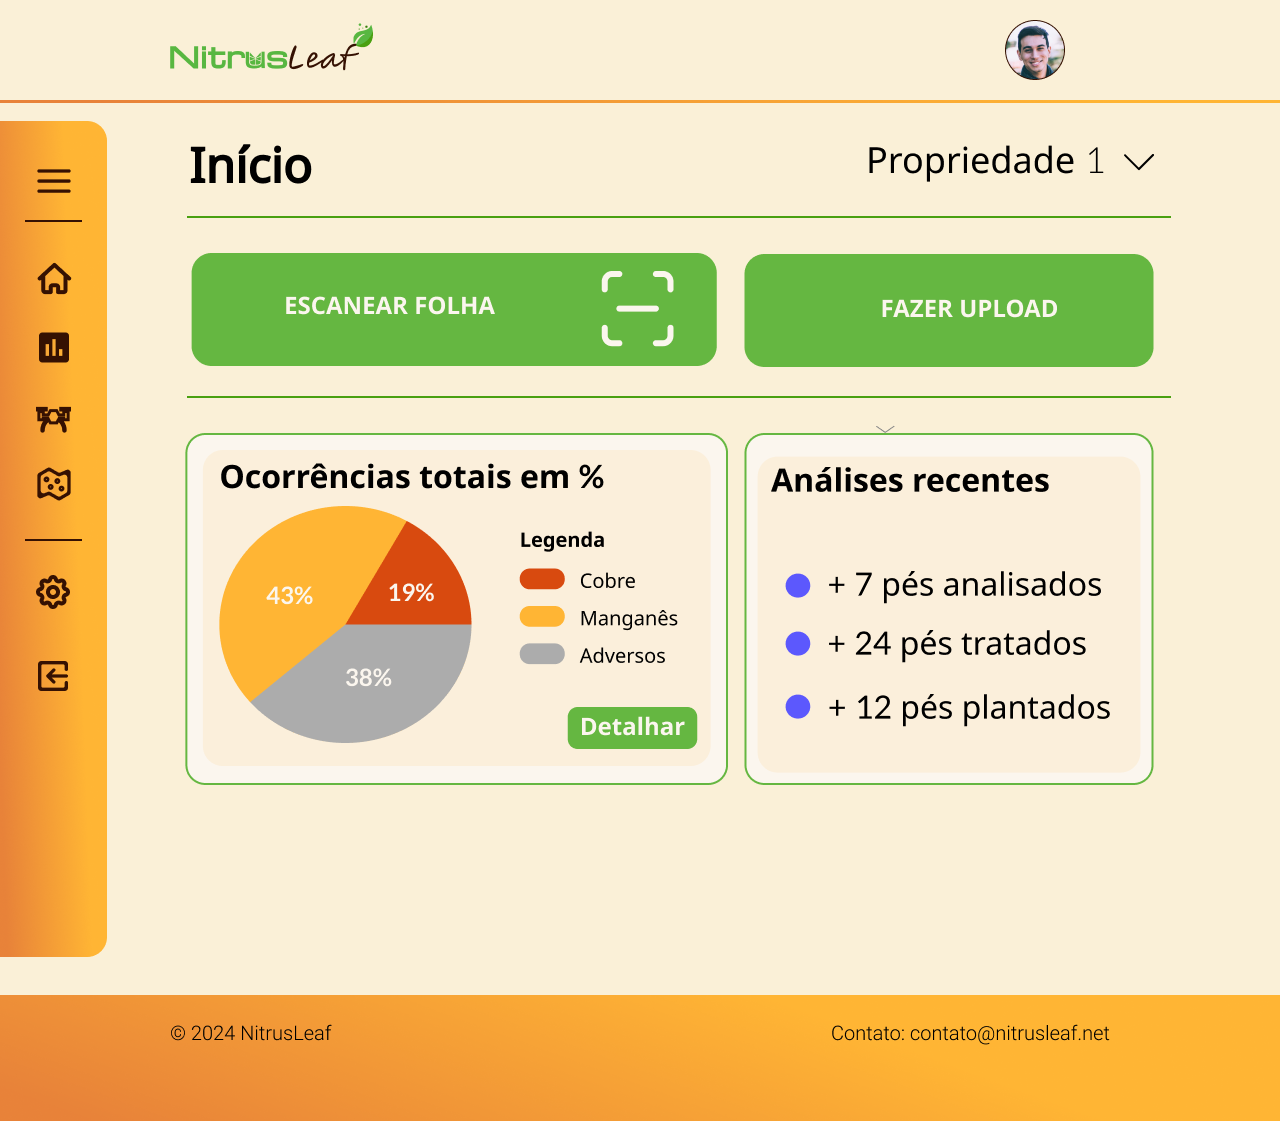
\includegraphics[width=0.7\linewidth]{Illustrations/tela-inicios.png}
\label{fig:tela-inicio}
\SourceOrNote{Autoria Própria (2024)}
\end{figure}

Ao selecionar “escanear folha”, o usuário deverá apontar a câmera para a folha escolhida. Caso opte por fazer o upload de uma imagem, o aplicativo iniciará a análise e, ao concluir, abrirá a tela \Cref{fig:cadastro-diagnóstico} mostrando a probabilidade da deficiência identificada. O usuário deve selecionar a planta analisada, o talhão ao qual pertence e pode adicionar um relatório, se necessário, antes de finalizar.

\begin{figure}[H]
\centering
\caption{Cadastro Diagnóstico}
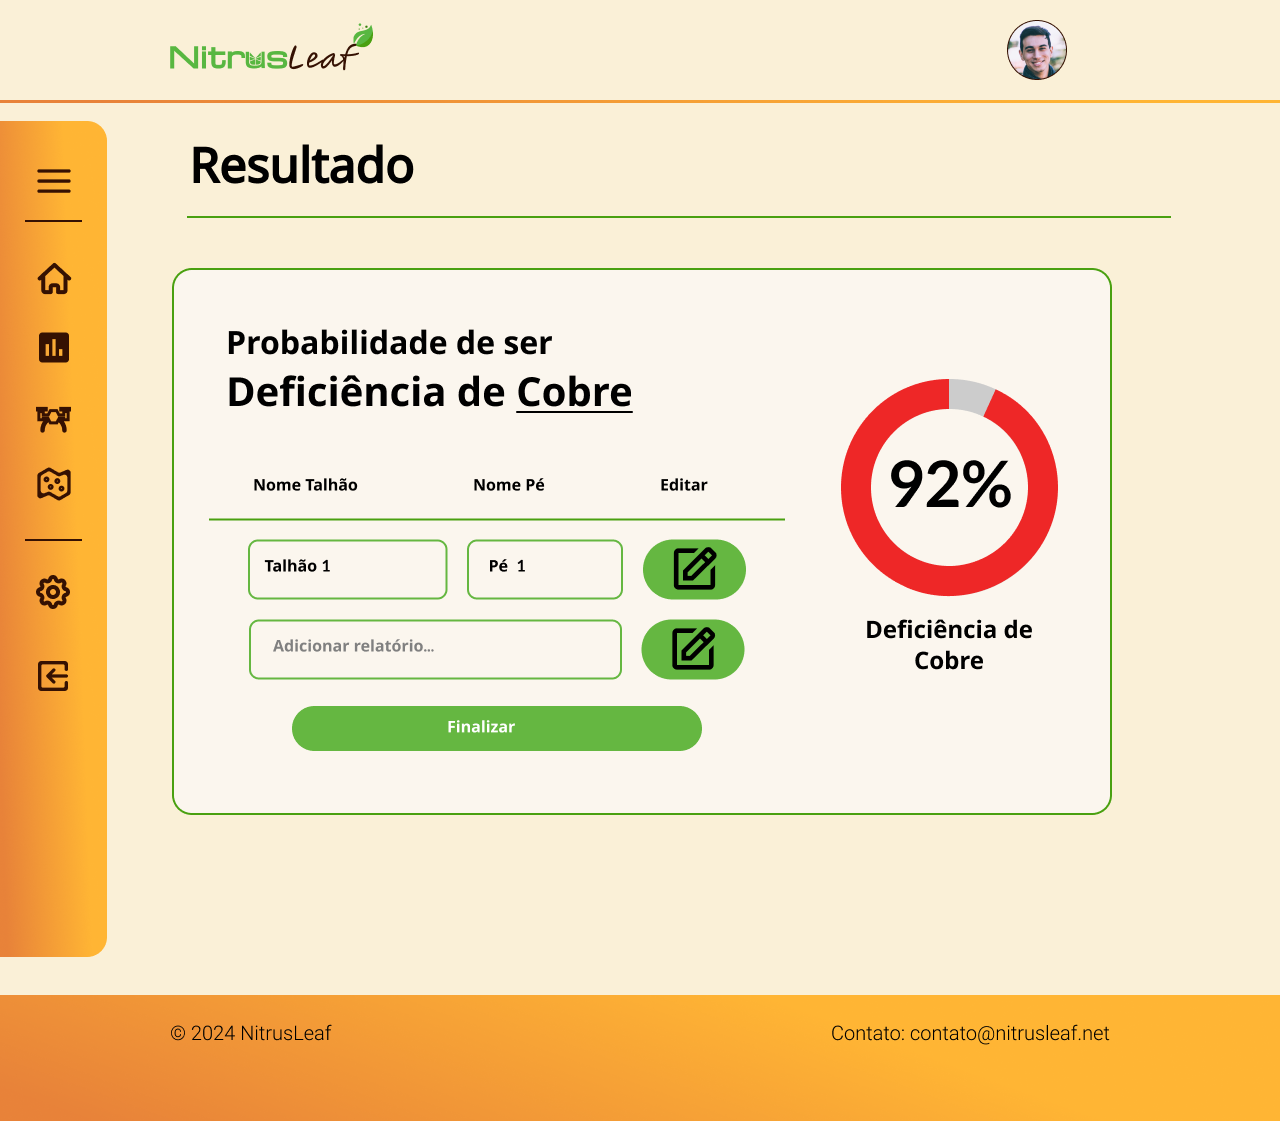
\includegraphics[width=0.8\linewidth]{Illustrations/Tela-Escaneamentos.png}
\label{fig:cadastro-diagnóstico}
\SourceOrNote{Autoria Própria (2024)}
\end{figure}

Para verificar as plantas cadastradas no aplicativo, o usuário acessa a tela de histórico \Cref{fig:tela-relatorios}. Nessa tela, é possível ver a quantidade de plantas cadastradas em cada talhão, selecionar a propriedade sendo verificada, bem como visualizar o número de plantas analisadas até o momento. No lado direito, uma janela exibe o total de talhões e plantas registrados, além do número de plantas analisadas e diagnosticadas.

\begin{figure}[H]
\centering
\caption{Tela Relatórios}
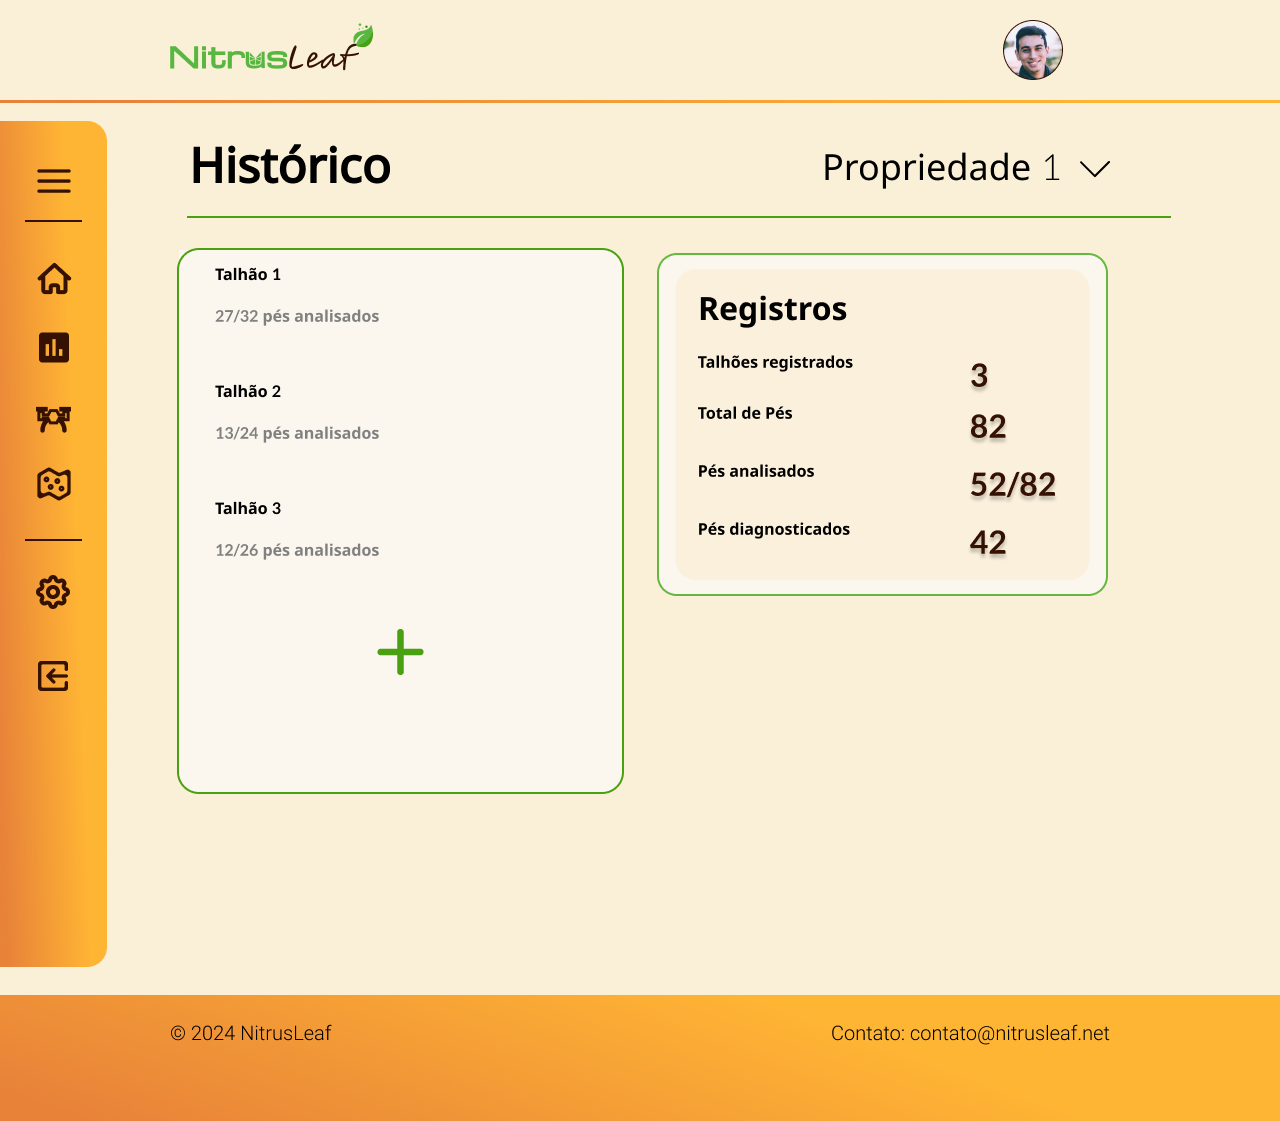
\includegraphics[width=0.7\linewidth]{Illustrations/tela-historico.png}
\label{fig:tela-relatorios}
\SourceOrNote{Autoria Própria (2024)}
\end{figure}

Na tela de mapas \Cref{fig:tela-mapas}, o usuário pode escolher entre diferentes tipos de mapas, como o NDVI, um mapa via satélite que mostra a localização, um mapa com todas as mexericas e um mapa de calor que exibe a concentração de possíveis deficiências.

O NDVI, ou Índice de Estado de Vegetação, é gerado a partir de imagens capturadas por drones e um gráfico de linhas que mostra o nível de NDVI para cada talhão ao longo de 12 meses. Esse índice mede a quantidade de energia refletida e absorvida pelas plantas, fornecendo informações sobre sua saúde com base nessa refletância. A luz visível (400 a 720 nm) é absorvida, enquanto o infravermelho próximo (720 a 1100 nm) é refletido em maior intensidade por plantas saudáveis. Plantas em estresse, desidratadas ou doentes absorvem mais luz infravermelha, o que afeta seu índice NDVI. Esse valor é calculado usando a fórmula: \textit{NDVI} = \((\text{NIR} - \text{VIS}) / (\text{NIR} + \text{VIS})\) \cite{ResultadoNDVIArtigo, ResultadoNDVISite}.

\begin{figure}[H]
\centering
\caption{Mapas}
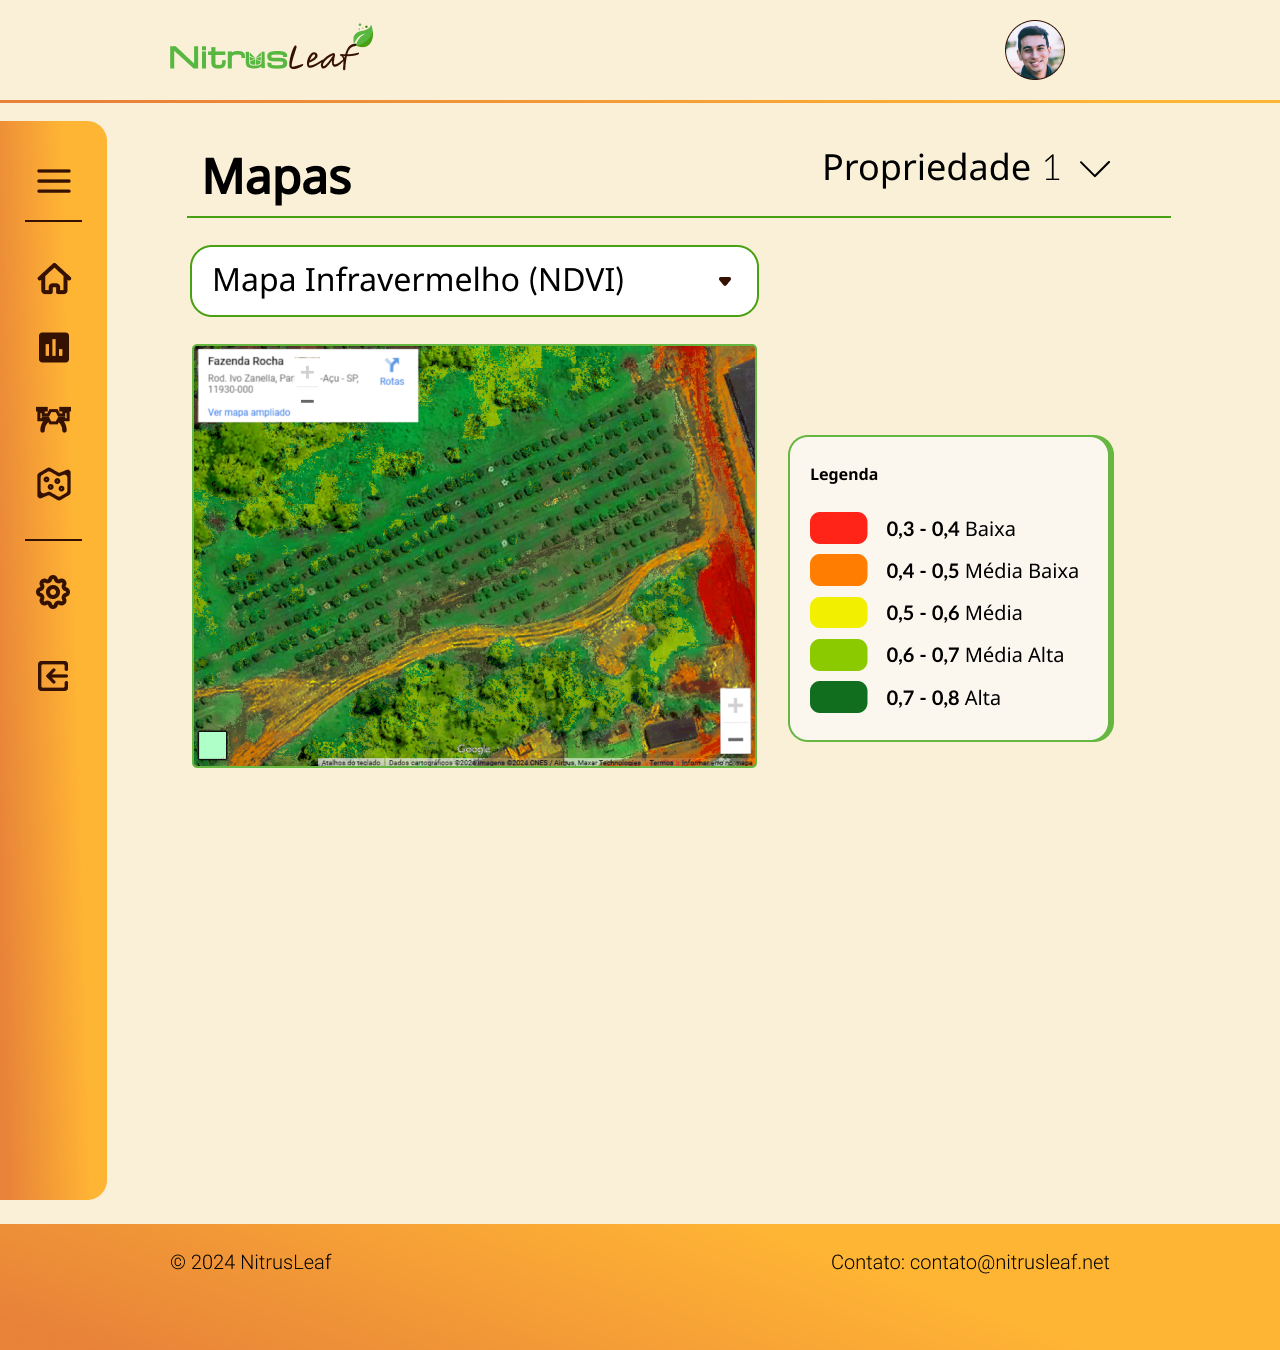
\includegraphics[width=0.7\linewidth]{Illustrations/tela-mapas.png}
\label{fig:tela-mapas}
\SourceOrNote{Autoria Própria (2024)}
\end{figure}

\textbf{Diagrama de classes}

O diagrama de classes do nosso projeto \Cref{fig:diagrama-classe} começa com a Landing Page, que é a tela inicial exibida caso o usuário não esteja logado. Nessa tela, o usuário pode optar por fazer login ou cadastrar-se. A tela de login permite que o usuário insira seu e-mail ou telefone celular e senha, com a opção de recuperação de senha, caso necessário.

O processo de cadastro envolve a inserção de dados como nome, sobrenome, e-mail, senha, telefone celular, confirmação de senha e endereço. Após essa etapa, o usuário pode continuar o cadastro, especificando o tipo de pessoa (física ou jurídica), CPF ou CNPJ (dependendo do tipo), logradouro, número, bairro e cidade. Em seguida, o sistema permite que o usuário cadastre sua propriedade, incluindo informações como nome, CEP, logradouro, número, bairro e cidade da propriedade. Esse cadastro de propriedade possibilita também a edição de talhões, permitindo ao usuário adicionar o nome do talhão e o nome do pé, com opções de edição ou finalização do cadastro.

Ao escolher escanear uma folha ou fazer o upload de uma imagem, o sistema realiza a análise da imagem e exibe uma tela de resultado que mostra a probabilidade de deficiência identificada ou outras condições. O usuário pode então informar o nome do pé analisado, o talhão ao qual ele pertence e, se necessário, adicionar um relatório à análise. O sistema permite editar o nome do pé, o talhão ou o relatório da análise antes de finalizar o cadastro do resultado.

Há também uma funcionalidade de histórico da propriedade, onde o usuário pode selecionar uma propriedade específica ou alternar para outro talhão, além de adicionar novos talhões. Ao escolher um talhão, o usuário consegue visualizar todos os pés cadastrados nele, podendo buscar um pé pelo nome, selecionar qualquer um dos pés, editar o talhão ou adicionar novos pés. Caso um pé específico seja selecionado, o usuário pode editar o nome, o relatório e, se necessário, excluí-lo do sistema.

\begin{figure}[H]
\centering
\caption{Diagrama de Classe}
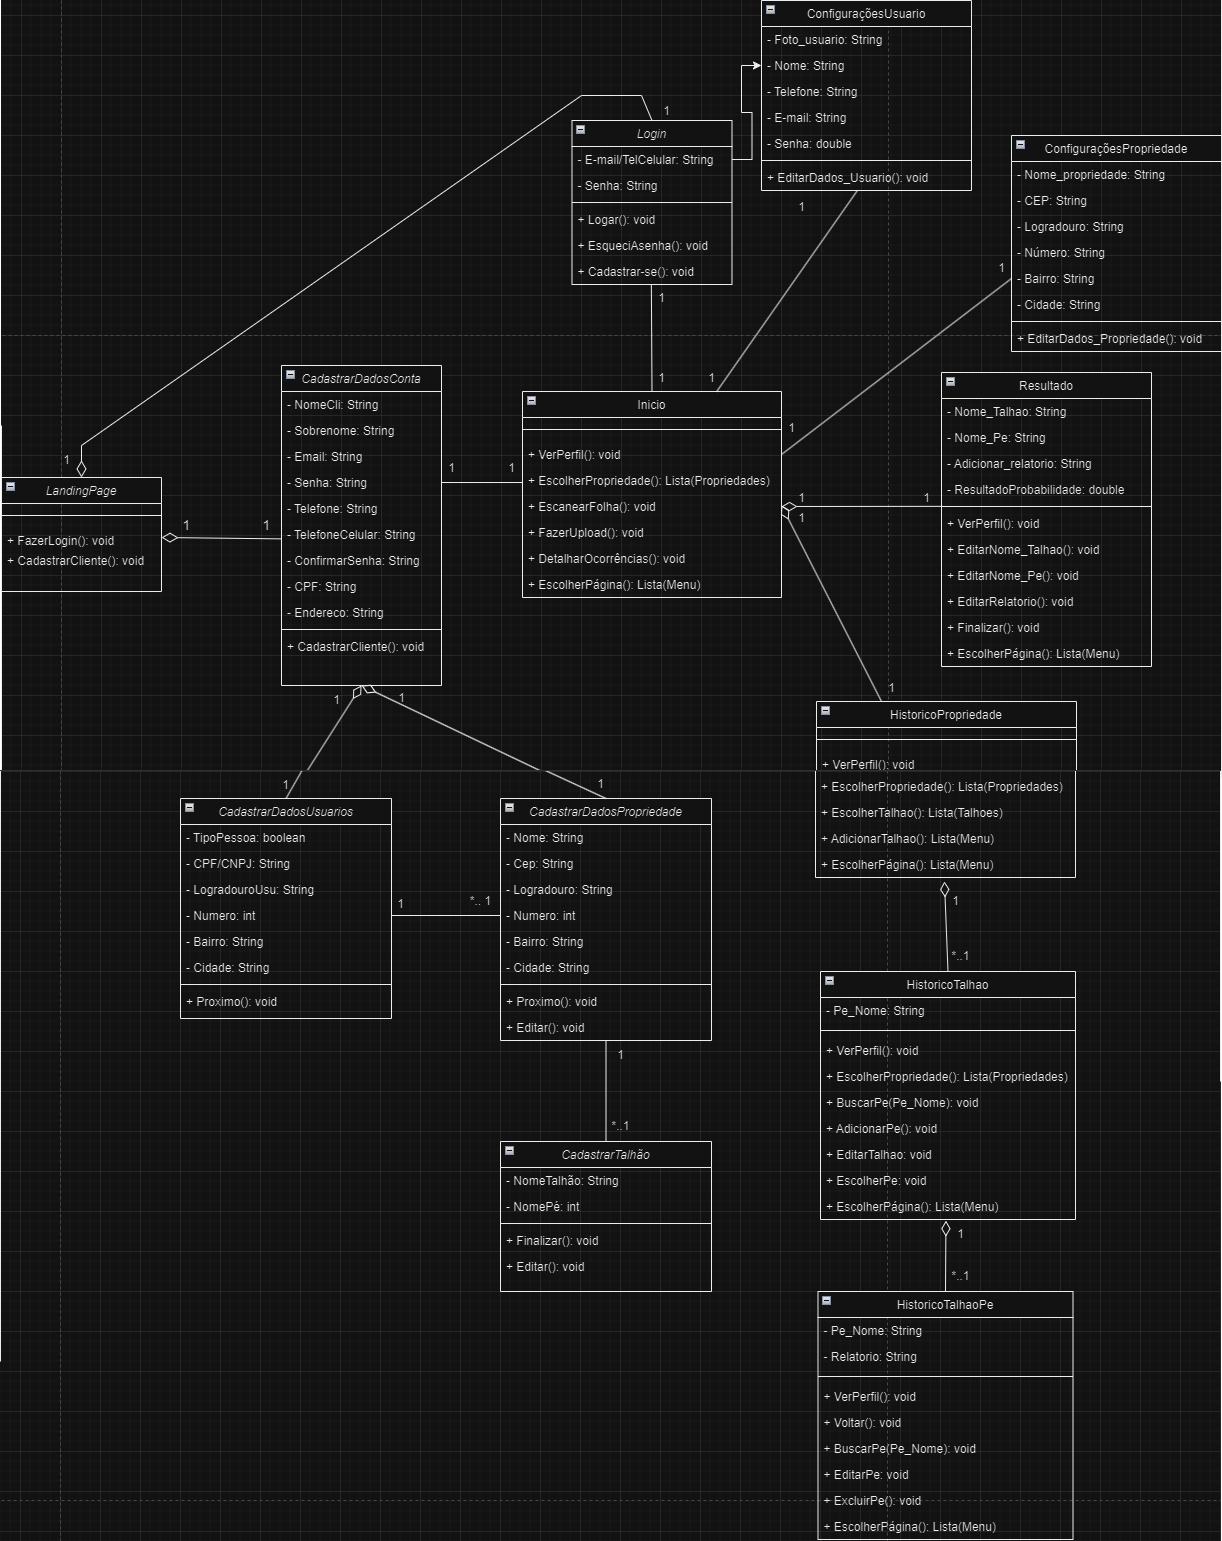
\includegraphics[width=0.7\linewidth]{Illustrations/diagramaClasse.png}
\label{fig:diagrama-classe}
\SourceOrNote{Autoria Própria (2024)}
\end{figure}

